\chapter{Mikrofonverstärker}

\begin{figure}[H]
    \centering
    \includegraphics[width = \textwidth]{tex/1_Microphone/pictures/Schaltung.png}
    \caption{verwendete Schaltung}
\end{figure}

\section{Berechnung und Dimensionierung}
\subsection{Berechnung der Widerstände}
\subsubsection{Gegebene Randbedingungen}

\begin{itemize}
    \item Spannung an $R_E$: \SI{2}{\volt}
    \item Innenwiderstand der Signalquelle: \SI{4.7}{\kilo \ohm}
    \item Basisquerstrom $I_q$: \SI{0.1}{\milli \ampere} \ldots \SI{1}{\milli \ampere}
    \item Spannung am Emitter des zweiten Transistors: \SI{5}{\volt}
\end{itemize}

\subsubsection{Berechnung von $R_1$ und $R_2$}

Der Basisquerstrom wird durch die Widerstände $R_1$ und $R_2$ bestimmt (Der Basisstrom wird als vernachlässigbar klein gegenüber dem Querstrom angenommen).

\begin{equation*}
    I_q = \SI{0.5}{\milli \ampere} = \frac{U_0}{R_1 + R_2} \rightarrow R_1 + R_2 = \frac{U_0}{I_q} = \SI{18}{\kilo \ohm}
\end{equation*}

Weiters ist bekannt, dass an der Basis des BC550 etwa \SI{2.7}{\volt} anliegen (Emitterspannung + PN-Übergang). 

\begin{equation*}
    U_{B,0} = \SI{2.7}{\volt} = U_0 \frac{R_2}{R_1+R_2} \rightarrow \frac{R_2}{R_1+R_2} = \frac{U_{B,0}}{U_0} = \frac{2.7}{9} = 0.3
    \rightarrow R_1 = 2.3 \ R_2
\end{equation*}

In einer ersten Abschätzung ergeben sich somit folgende Werte für $R_1$ und $R_2$:

\begin{equation*}
    R_1 = \SI{12.545}{\kilo \ohm} \quad R_2 = \SI{5.454}{\kilo \ohm}
\end{equation*}

Gerundet auf die nähestenden Werte der E24-Reihe ergeben sich Widerstandswerte von:

\begin{equation*}
    R_1 = \SI{13}{\kilo \ohm} \quad R_2 = \SI{5.6}{\kilo \ohm}
\end{equation*}

Dies führt zu folgenden Schaltungsparametern:

\begin{equation*}
    I_q = \SI{484}{\milli \ampere} \quad U_{B,0} = \SI{2.710}{\volt}
\end{equation*}

In dieser Berechnung wurden einige Vereinfachungen durchgeführt, wie zutreffend dieses Ergebnis ist, muss durch die Simulation geprüft werden.

\subsubsection{Abschätzung des idealen Kollektorstroms}

Der optimale Kollektorstrom für einen möglichst rauscharmen Verstärker wird mit Gleichung 2.1 aus dem Praktikumsskript bestimmt:

\begin{equation*}
    R_0 = \sqrt{\frac{2 \ \beta \  r_{BB}}{I_{C0}}U_T + \frac{\beta}{ {I_{C0}}^2 }U_{T}^2}
\end{equation*}

umgeformt auf den gesuchten Strom ergibt sich:

\begin{align*}
    0 &= R_0^2 I_{C0}^2 - 2 \ \beta  r_{BB}  U_T  I_{C0} - \beta U_{T}^2 \\
    I_{C0} &= \frac{2 \ \beta  r_{BB}  U_T \pm \sqrt{\left( 2 \ \beta  r_{BB}  U_T\right)^2 + 4  R_{0}^2 \beta U_{T}^2 }}{2 R_{0}^2} \\
    I_{C0} &= U_T \frac{ \ \beta  r_{BB} \pm \sqrt{ \beta^2  r_{BB}^2 +  R_{0}^2 \beta }}{ R_{0}^2} \\
    I_{C0} &= \SI{25}{\milli \volt} \frac{600 \cdot \SI{150}{\ohm} \pm \sqrt{(600 \cdot \SI{150}{\ohm})^2 + (\SI{2136}{\ohm})^2 \cdot 600}}{(\SI{2136}{\ohm})^2} = \SI{1.064}{\milli \ampere}, \SI{-77.28}{\micro \ampere}
\end{align*}

Das negative Ergebnis für $I_{C0}$ wird als nicht-physikalisch interpretiert und verworfen, weitergerechnet wird mit $I_{C0} = \SI{1}{\milli \ampere}$

Verwendeete Werte:

\begin{itemize}
    \item Kleinsignalverstärkung des BC550C \emph{typ.: }$\beta = 600$
    \item Basisbahnwiderstand \emph{Base Spreading Resistance}: $r_{BB} \approx \SI{150}{\ohm}$ \\
    Anm.: $r_{BB}$ ist eine funktion von $I_{C0}$, dieser Wert gilt für ca. \SI{3}{\milli\ampere}, bei großer Abweichung muss iterativ eingesetzt werden.
    \item Temperaturspannung: $U_T = \frac{k_b T}{e} = \SI{25}{\milli \volt}$ \\
    Anm.: Dieser Wert gilt bei Raumtemperatur, je nach Temperatur bzw. Verlustleistung des Transistors ist dieser Wert zu hinterfragen.
    \item Generatorwiderstand $R_0 = \left( G_1 + G_2 + G_G\right)^{-1} = \SI{2136}{\ohm}$
\end{itemize}

\subsubsection{Berechnung von $R_E$ und $R_C$}

Durch $R_E$ und $R_C$ fließen im wesentlichen der eben berechnete Kollektorstrom (der Basisstrom wird vernachlässigt).

\begin{equation*}
    U_{R_{E}} = \SI{2}{\volt} = I_{C0} R_E \rightarrow R_E = \SI{2}{\kilo \ohm}
\end{equation*}

Der Kollektor des ersten Transistors ist an der Basis des zweiten Transistors angeschlossen. Dessen Emitter soll auf einem Potential von etwa \SI{5}{\volt} liegen. Damit liegt die Basis dieses zweiten Transistors auf \SI{5.7}{\volt}.

\begin{equation*}
    \SI{9}{\volt} - \SI{5.7}{\volt} = I_{C0} R_C \rightarrow R_C = \SI{3.3}{\kilo \ohm}
\end{equation*}

\subsection{Abschätzung von Ein- und Ausgangswiderstand}

Zur Abschätzung der Betriebsparameter wie Eingangswiderstand $r_e$ und Ausgangswiderstand $r_a$ muss das Kleinsignalersatzschaltbild (KSESB) ausgewertet werden.

\begin{figure}[H]
    \centering
    \includegraphics[width = \textwidth]{tex/1_Microphone/pictures/KSESB.pdf}
    \caption{Kleinsignalersatzschaltbild der Schaltung}
    \label{fig:my_label}
\end{figure}

\subsubsection{Eingangswiderstand}

\begin{equation*}
    r_e = \left.\frac{u_e}{i_e}\right|_{R_L}
\end{equation*}

Aus den Anmerkungen zur Auslegung der Koppelkondensatoren ist zu entnehmen dass es ausreichend ist die Grenzfälle $\omega \rightarrow 0$ und $\omega \rightarrow \infty$ bzw. den worst case zu betrachten.

Im DC-Fall ($\omega \rightarrow 0$), sperrt der Kondensator $C_1$ und der Eingangswiderstand ist im eingeschwungenen Zustand sehr hoch. In der Praxis jedoch nicht unendlich (Leckströme und andere parasitäre Effekte). Zur Abschätzung des worst-case $r_{e,\text{min}}$ wird also der hochfrequente Fall ($\omega \rightarrow \infty$) betrachtet.

Analog wie im Übungsskriptum werden die Koppelkondensatoren $C_1$ und $C_2$ durch einen Kurzschluss ersetzt und der Emitterkondensator $C_E$ durch einen Leerlauf. Weiters wird der Earlywiderstand vernachlässigt, in der späteren Simulation wird sich zeigen ob dies gerechtfertigt ist.

Es ergibt sich folgende Gleichung:

\begin{equation*}
    U_e = \underbrace{\left( i_e - \frac{U_e}{R_1 || R_2}\right)}_{i_B} \left( r_{BE} + R_E \left( B + 1\right) \right)
\end{equation*}

\begin{equation*}
    U_e = i_e \left( r_{BE} + R_E \left( B + 1\right) \right) - U_e \frac{r_{BE} + R_E \left( B + 1\right)}{R_1 || R_2}
\end{equation*}

\begin{equation*}
    U_e \left( 1 + \frac{r_{BE} + R_E \left( B + 1\right)}{R_1 || R_2}) \right)= i_e \left( r_{BE} + R_E \left( B + 1\right) \right)
\end{equation*}

\begin{equation*}
    r_e = \frac{u_e}{i_e} = \frac{r_{BE} + R_E \left( B + 1\right)}{ 1 + \frac{r_{BE} + R_E \left( B + 1\right)}{R_1 || R_2} }= \SI{3901.42}{\ohm} \approx R_1 || R_2
\end{equation*}

\begin{equation*}
    C_E = \frac{S}{2 \pi f_G} = \frac{\SI{1}{\milli \ampere}}{2 \pi \ \SI{57.735}{\hertz} \ \SI{25}{\milli \volt}} = \SI{110.3}{\micro \farad}
\end{equation*}

\begin{equation*}
   r_{BE} = \frac{B}{S} = \frac{600}{\frac{\SI{1}{\milli \volt\ampere}}{\SI{25}{\milli\volt}}} = \SI{15}{\kilo \ohm} 
\end{equation*}

\subsubsection{Ausgangswiderstand}

\begin{equation*}
    r_a = \left. - \frac{u_a}{i_a}\right|_{R_G, U_G = 0}
\end{equation*}

Zur Berechnung des Ausgangswiderstandes muss ein leicht verändertes KSESB verändert werden:

\begin{figure}[H]
    \centering
    \includegraphics[width = \textwidth]{tex/1_Microphone/pictures/KSESB_ra.pdf}
    \caption{Kleinsignalersatzschaltbild der Schaltung zur Berechnung des Ausgangswiderstandes}
    \label{fig:my_label}
\end{figure}

Der Ausgangswiderstand wird maßgeblich durch die Stellung des Potentiometers $P_1$ beeinflusst. Um dies zu verdeutlichen wird das Potentiometer in 2 Widerstände ($P_{1,1}$ und $P_{1,2}$) aufgeteilt:

\begin{figure}[H]
    \centering
    \includegraphics[width = 0.5\textwidth]{tex/1_Microphone/pictures/ra_spannungsteiler.pdf}
    \caption{Ausgangsspannungsteiler im Detail}
    \label{fig:my_label}
\end{figure}

In einer ungünstigen Potistellung wird der Widerstand $P_{1,2}$ zu \SI{0}{\ohm} und der Ausgangswiderstand ebenfalls zu \SI{0}{\ohm}. Dies ist der minimale Ausgangswiderstand $R_{a,\text{min}}$. Dieser Fall ist jedoch nicht von besonderen Interesse, da hier der Lastwiderstand defacto mit beiden Polen an Masse liegt und kein Teil der Schaltung mehr ist.

Überlegungen zur Schaltungsvereinfachung:

Da es sich hier nur um eine grobe Abschätzung handelt, die später mittels Simulation verifiziert wird, werden die (ohnehin noch nicht dimensionierten) Kondensatoren und Early-Widerstände nicht berücksichtigt.

\begin{figure}[H]
    \centering
    \includegraphics[width = \textwidth]{tex/1_Microphone/pictures/KSESB_simplified.pdf}
    \caption{Kleinsignalersatzschaltbild der Schaltung zur Berechnung des Ausgangswiderstandes}
    \label{fig:my_label}
\end{figure}

Aus Masche 1 ergibt sich, dass der Basisstrom des ersten Transistors verschwindet:

\begin{equation*}
    M1: \quad i_b \left( R_1 || R_2 || R_G + r_{BE} + (B + 1) R_E\right) = 0 \rightarrow i_b = 0
\end{equation*}

Der Strom $i_a$ fließt also nur durch die Widerstände $P_1$, $r_{BE}$ (des zweiten Transistors) und $R_C$:

\begin{figure}[H]
    \centering
    \includegraphics[width = 0.55\textwidth]{tex/1_Microphone/pictures/KSESB_ra_detail.pdf}
    \caption{Kleinsignalersatzschaltbild der Schaltung zur Berechnung des Ausgangswiderstandes}
    \label{fig:my_label}
\end{figure}


\begin{align*}
    M_1:& \quad i_b(R_C + r_{BE} + (B+1) P_{1,1}) + P_{1,2} i_1= 0 \\
    M_2:& \quad U_a = P_{1,2} i_1 \\
    M_3:& \quad P_{1,1} (i_b (B+1)) = U_a\\
    K_2:& \quad i_b (B+1) - i_1 = i_a
\end{align*}

Nach einigen Umformungen folgt:

\begin{align*}
    M_1:& \quad i_b(R_C + r_{BE} + (B+1) P_{1,1}) + U_a= 0 \\
    & \quad i_b = \frac{-U_a}{R_C + r_{BE} + (B+1) P_{1,1}}\\
    M_2:& \quad i_1 = \frac{U_a }{ P_{1,2}} \\
    M_3:& \quad P_{1,1} (i_b (B+1)) = U_a\\
    K_2:& \quad i_b (B+1) - \frac{U_a }{ P_{1,2}} = i_a \\
        & \quad - \frac{U_a}{R_C + r_{BE} + (B+1) P_{1,1}}(B+1) - \frac{U_a }{ P_{1,2}} = i_a \\
        & \quad - U_a \left( \frac{B+1}{R_C + r_{BE} + (B+1) P_{1,1}} + \frac{1}{P_{1,2}} \right) = i_a \\
        r_a &= -\frac{U_a}{i_a} = \frac{1}{\left( \frac{B+1}{R_C + r_{BE} + (B+1) P_{1,1}} + \frac{1}{P_{1,2}} \right)} = P_{1,2} || \left( P_{1,1} + \underbrace{\frac{R_C + r_{BE}}{B+1}}_{\approx \SI{22}{\ohm}}\right)
\end{align*}

Im wesentlichen ist der Ausgangswiderstand nur von der Potentiometerstellung abhängig, da der andere Teil durch die Stromverstärkung $B$ stark abgedämpft wird und kaum Auswirkung hat.

Ein typischer Wert von B für den zweiten Transistor lautet 330. Die Größe des $r_{BE}$ hängt von der verwendeten Last ab. Wenn die Schaltung ohne Last betrieben wird, ergibt sich ein Emitterstrom von etwa \SI{2.2}{\milli \ampere}, dies entspricht auch etwa dem Kollektorstrom und mit diesem Wert wird $r_{BE}$ berechnet:

\begin{equation*}
    r_{BE} = \frac{B}{S} = \frac{330}{\frac{I_{C0}}{U_T}} = \frac{330 U_T}{\SI{2.2}{\milli \ampere}} = \SI{3.75}{\kilo \ohm}
\end{equation*}

\subsubsection{Ausgangswiderstand als Funktion der Potistellung}

Mit dem gefundenen Ausdruck für $r_a$, lässt sich dieser als Funktion der Potentiometerstellung $\frac{P_{1,1}}{P_{1,1}+P_{1,2}}$ darstellen:

\begin{figure}[H]
    \centering
    \includegraphics[width = 0.55\textwidth]{tex/1_Microphone/pictures/simple_plot.pdf}
    \caption{Ausgangswiderstand als Funktion der Potistellung}
    \label{fig:my_label}
\end{figure}

Der maximale Ausgangswiderstand von \SI{555}{\ohm} wird bei einer mittleren Potentiometerstellung erreicht. Wenn der Widerstand $P_{1,1}$ auf \SI{0}{\ohm} gestellt wird, wird $r_a$ zu \SI{21}{\ohm} (Der durch die Stromverstärkung abgedämpfte Term wird dominant).

\subsection{Dimensionierung der Kapazitäten}

Die Berechnung der Kapazitäten wurden aus dem beigelegten Dokument \glqq Anmerkung zur Auslegung der Koppelkondensatoren beim Mikrofonverstärker\grqq{} übernommen:

\begin{equation*}
    C_1 = \frac{1}{2 \pi f_G \left( R_G + r_{E,\text{min}} \right)} = \frac{1}{2 \pi \SI{57.735}{\hertz} \left(\SI{4.7}{\kilo \ohm} +  \SI{3901}{\ohm}\right)} = \SI{320}{\nano \farad} \rightarrow \SI{300}{\nano \farad}
\end{equation*}

Bei der dimensionierung von $C_2$ ist der minimale Ausgangswiderstand der Schaltung relevant, da sich die Zeitkonstante $\tau = RC$ mit sinkenden Widerstand absenkt, niedrigere Zeitkonstante gleich niedrigere Grenzfrequenz. Bei diesem Hochpass besteht die Gefahr, dass die Grenzfrequenz zu hoch liegt, also muss man mit dem minimalen Widerstand dimensionieren.

\begin{equation*}
    C_2 = \frac{1}{2 \pi f_G \left( r_{a,\text{min}} + r_{L,\text{min}} \right)} = \frac{1}{2 \pi \SI{57.735}{\hertz} \left(\SI{21}{\ohm} +  \SI{1}{\kilo \ohm}\right)} = \SI{2.7}{\micro \farad} \rightarrow \SI{2.7}{\micro \farad}
\end{equation*}

\begin{equation*}
    C_E = \frac{S}{2 \pi f_G} = \SI{110.3}{\micro \farad} \rightarrow \SI{110}{\micro \farad}
\end{equation*}

\subsection{Bestimmung der maximalen Spannungsverstärkung}

Im Allgemeinen wird die Spannungsverstärkung eine Funktion der Frequenz $f$, der Potentiometerstellung und dem Lastwiderstand (es wird nicht explizit von der Leerlaufverstärkung gesprochen) sein.
Zur Vereinfachung wird angenommen, dass die Schaltung in einem Bereich betrieben wird, in dem die Kapazitäten $C_1$ und $C_2$ durch Kurzschlüsse ersetzt werden können.

Weiters soll die Berechnung einmal mit dem Kondensator $C_E$ und einmal ohne durchgeführt werden.

Zur Berechnung der Gesamtspannungsverstärkung wird versucht diesen zweistufigen Verstärker als Kaskadierung zweier unabhängiger Verstärker zu betrachten: 

\subsubsection{Berechnung ohne $C_E$}

\begin{figure}[H]
    \centering
    \includegraphics[width = 0.55\textwidth]{tex/1_Microphone/pictures/KKSESB_ohne_CE.pdf}
    \caption{Kleinsignalersatzschaltbild der ersten Stufe ohne $C_E$}
    \label{fig:my_label}
\end{figure}

Gesucht ist folgender Ausdruck: $\frac{U_{E,2}}{U_E}$

\begin{align*}
    M_1:& \quad U_E = i_b \left( r_{BE} + R_E \left( B + 1\right) \right) \\
    M_2:& \quad R_E i_b (B+1) + R_C i_b B = 0 \\
    {} & \quad U_{BE} = i_b r_{BE} = U_E \frac{r_{BE}}{r_{BE}+R_E(B+1)}\\
    {} & \quad r_{BE} \approx \frac{B}{S}\\
    {} & \quad U_{E,2} = - S U_{BE} R_C = - U_E R_C \frac{B}{\frac{B}{S}+S R_E(B+1)}\\
    & \quad \frac{U_{E,2}}{U_E} = - R_C \frac{B}{\frac{B}{S}+S R_E(B+1)} = -31.39
\end{align*}

\subsubsection{Berechnung mit $C_E$}

\begin{figure}[H]
    \centering
    \includegraphics[width = 0.55\textwidth]{tex/1_Microphone/pictures/KKSESB_mit_CE.pdf}
    \caption{Kleinsignalersatzschaltbild der ersten Stufe mit $C_E$}
    \label{fig:my_label}
\end{figure}

Die Kapazität $C_E$ schließt den Widerstand $R_E$ im Kleinsignalbetrieb kurz.

Gesucht ist folgender Ausdruck: $\frac{U_{E,2}}{U_E}$

\begin{align*}
    M_1:& \quad U_E = U_{BE} \\
    & \quad U_{E,2} = - S U_{BE} R_C = - U_E S R_C \\
    {} & \quad  \frac{U_{E,2}}{U_E} = - S R_C = -132 \\
\end{align*}

\subsubsection{Berechnung der zweiten Verstärkerstufe}

\begin{figure}[H]
    \centering
    \includegraphics[width = 0.55\textwidth]{tex/1_Microphone/pictures/KSESB_second_stage.pdf}
    \caption{Kleinsignalersatzschaltbild der zweiten Stufe}
    \label{fig:my_label}
\end{figure}

Bei der zweiten Stufe (Kollektorschaltung) wird eine Verstärkung von 1 erwartet.

\begin{align*}
    M_1:& \quad U_E = i_b \left( r_{BE} + (B+1) (P_{1,1} + P{1,2} || R_L) \right) \\
    & \quad i_b = U_E \frac{1}{\left( r_{BE} + (B+1) (P_{1,1} + P{1,2} || R_L) \right)} \\
    \\
    & \quad U_a =  U_E \frac{(B+1) (P_{1,1} + P{1,2} || R_L)}{r_{BE} + (B+1) (P_{1,1} + P{1,2} || R_L)} \\
    & \quad \frac{U_a}{U_E} = \frac{(B+1) (P_{1,1} + P{1,2} || R_L)}{ r_{BE} + (B+1) (P_{1,1} + P{1,2} || R_L)} \leq 1\\
\end{align*}

Für vernünftige Lastwiderstände und Potentiometerstellungen (als unvernünftig gilt hier ein Kurzschluss des Emitters gegenüber Masse) geht diese Verstärkung gegen 1.

\emph{Erkentniss zu den Verstärkungen:} Hohe Frequenzen werden höher verstärkt als niedrige Frequenzen. Die tatsächliche Verstärkung liegt zwischen $\approx 30$ und $\approx 130$.

\subsection{Auswirkungen der Temperatur auf die Arbeitspunktströme}

Zur Bestimmung des Werts $\frac{\Delta U_{BE}}{\Delta T}$ wird eine Simulation, wie in Abschnitt 2.3.3 des Praktikumsskripts erläutert, durchgeführt.
Es wird ein Kollektorruhestrom von \SI{1.064}{\milli \ampere} eingestellt und ein Widerstand gewählt, so dass sich $U_{CE}$ zu \SI{3.56}{\volt} ergibt.

\begin{figure}[H]
    \centering
    \includegraphics{tex/1_Microphone/pictures/Aufbau, Tempsimulation.png}
    \caption{Simulationsaufbau}
    \label{fig:my_label}
\end{figure}

Dies wird erreicht bei einem Widerstand von \SI{638}{\kilo \ohm}

Die Simulation ergab folgenden (annähernd linearen) Zusammenhang zwischen $U_{BE}$ und der Temperatur:

\begin{table}[H]
    \centering
    \begin{tabular}{|c|c|}
    \hline
         Temperatur & $U_{BE}$  \\ \hline \hline
         \SI{-20}{\celsius}& \SI{743.42}{\milli \volt} \\ \hline
         \SI{-10}{\celsius}& \SI{726.46}{\milli \volt} \\ \hline
         \SI{0}{\celsius}& \SI{709.41}{\milli \volt} \\ \hline
         \SI{10}{\celsius}& \SI{692.26}{\milli \volt} \\ \hline
         \SI{20}{\celsius}& \SI{675.02}{\milli \volt} \\ \hline
         \SI{30}{\celsius}& \SI{657.69}{\milli \volt} \\ \hline
         \SI{40}{\celsius}& \SI{640.27}{\milli \volt} \\ \hline
         \SI{50}{\celsius}& \SI{622.78}{\milli \volt} \\ \hline
         \SI{60}{\celsius}& \SI{605.20}{\milli \volt} \\ \hline
         \SI{70}{\celsius}& \SI{587.54}{\milli \volt} \\ \hline
         \SI{80}{\celsius}& \SI{569.81}{\milli \volt} \\ \hline
    \end{tabular}
    \caption{Zusammenhang Temperatur und $U_{BE}$}
    \label{tab:my_label}
\end{table}

gemittelt über den gesamten Bereich ergibt sich also folgender Temperaturkoeffizient für diesen Typ von Transistor und Arbeitspunkt:

\begin{equation*}
    \frac{\Delta U_{BE}}{\Delta T} = \frac{-\SI{743.42}{\milli \volt} + \SI{569.81}{\milli \volt}}{\SI{100}{\kelvin}} = \SI{-1.7361}{\milli \volt \per \kelvin}
\end{equation*}

Der, durch die Simulation gewonnene Wert, weicht also doch recht deutlich von den typischerweise Verwendeten \SI{-2}{\milli \volt \per \kelvin} ab.

\begin{figure}[H]
    \centering
    \includegraphics[width = 0.55\textwidth]{tex/1_Microphone/pictures/KSESB_temp.pdf}
    \caption{Kleinsignalersatzschaltbild der ersten Stufe mit berücksichtigter Temperatur}
    \label{fig:my_label}
\end{figure}

\begin{align*}
    M_1:& \quad U_E = \Delta U_{BE}(\Delta T) + i_b \left( r_{BE} + (B+1) R_E \right) \\
    & \quad i_b = (U_E - \Delta U_{BE}(\Delta T)) \frac{1}{r_{BE} + (B+1) R_E} \\
     & \quad \frac{\partial i_b}{\partial T} = -\frac{\partial \Delta U_{BE}(\Delta T)}{\partial T} \frac{1}{r_{BE} + (B+1) R_E}
     = \frac{\SI{1.7361}{\milli \volt \per \kelvin}}{r_{BE} + (B+1) R_E} = \SI{1.426}{\nano \ampere \per \kelvin}\\
    &  \quad \frac{\partial i_c}{\partial T} = B \frac{\partial i_b}{\partial T} = \SI{855}{\nano \ampere \per \kelvin} \approx \frac{\partial i_e}{\partial T}\\
\end{align*}

Die Ströme sind also tatsächlich sehr temperaturstabil.

\section{Simulation in LTSpice}

\subsection{Überprüfen der Arbeitspunkte}

\begin{table}[H]
    \centering
    \begin{tabular}{|c|c|c|}
    \hline
         Bezeichnung der Größe & errechneter/gewünschter Wert & simulierter Wert \\ \hline \hline
         Spannung an $R_E$ & $\SI{2}{\volt}$ & $\SI{2.030}{\volt}$ \\ \hline
         Basisquerstrom $I_q$ & $\SI{484}{\milli \ampere}$ & $\SI{485}{\milli \ampere}$ \\ \hline
         Spannung an der Basis des $T_1$ & $\SI{2.71}{\volt}$ & $\SI{2.69}{\volt}$ \\ \hline
         Kollektorstrom des ersten Transistors& \SI{1.064}{\milli \ampere} & \SI{1.032}{\milli \ampere} \\ \hline
         Spannung am Emitter des $T_2$ & \SI{5}{\volt} & \SI{4.798}{\volt} \\ \hline
         Kollektorstrom des $T_2$ & - & \SI{2.159}{\milli \ampere} \\ \hline
    \end{tabular}
    \caption{Vergleich der angepeilten und erreichten Werte}
    \label{tab:my_label}
\end{table}

Die gemessenen Werte wurden wie folgt gemessen:
\begin{itemize}
    \item Aufbau der Schaltung in LTSpice mit den errrechneten Werten für Widerstände und Kapazitäten
    \item Für den ersten Transistor wurde das Modell des BC 550C eingefügt, für den zweiten Transistor wurde ein generischer NPN verwendet.
    \item Die Eingangsspannungsquelle wurde auf \SI{10}{\milli \volt} (konstante Gleichspannung) gesetzt.
    \item Anschließend wurde die Schaltung eine Sekunde lang simuliert und danach die Werte aufgenommen.
\end{itemize}

\subsection{Dimension des minimalen Lastwiderstandes}

Auch bei ungünstigsten Potistellungen darf der Strom über das Potentiometer nicht über \SI{8.25}{\volt} ansteigen.
Im worst-case wird das Potentiometer beinahe vollständig vom Lastwiderstand überbrückt und bei einem Kurzschluss des Lastwiderstandes würde ein sehr hoher Strom über diese kurze Strecke des Potentiometers fließen $\rightarrow$ Zerstörung des Potentiometers!

Um dies zu vermeiden muss der Lastwiderstand auch bei maximaler Austeuerung den Strom auf \SI{8.25}{\milli \ampere} begrenzen. Die maximale Aussteuerung beträgt \SI{8}{\volt}, somit ist ein minimaler Lastwiderstand von \SI{970}{\ohm} notwendig.

\subsection{Simulation des Temperaturverhaltens}

Wenn man die Temperatur variiert und den Kollektorstrom des ersten Transistors beobachtet stellt man folgende Beobachtungen auf:

\begin{table}[H]
    \centering
    \begin{tabular}{|c|c|}
    \hline
         Temperatur & $I_{C}$  \\ \hline \hline
         \SI{-20}{\celsius}& \SI{967}{\micro \ampere} \\ \hline
         \SI{-10}{\celsius}& \SI{977}{\micro \ampere} \\ \hline
         \SI{0}{\celsius}& \SI{986}{\micro \ampere} \\ \hline
         \SI{10}{\celsius}& \SI{995}{\micro \ampere} \\ \hline
         \SI{20}{\celsius}& \SI{1004}{\micro \ampere} \\ \hline
         \SI{30}{\celsius}& \SI{1013}{\micro \ampere} \\ \hline
         \SI{40}{\celsius}& \SI{1022}{\micro \ampere} \\ \hline
         \SI{50}{\celsius}& \SI{1032}{\micro \ampere} \\ \hline
         \SI{60}{\celsius}& \SI{1041}{\micro \ampere} \\ \hline
         \SI{70}{\celsius}& \SI{1050}{\micro \ampere} \\ \hline
         \SI{80}{\celsius}& \SI{1059}{\micro \ampere} \\ \hline
    \end{tabular}
    \caption{Zusammenhang Temperatur und $I_{C}$ am BC550C}
    \label{tab:my_label}
\end{table}

gemittelt über den gesamten Bereich ergibt sich also folgender Temperaturkoeffizient für diesen Typ von Transistor und Arbeitspunkt:

\begin{equation*}
    \frac{\Delta I_{c}}{\Delta T} = \frac{\SI{1059}{\micro \ampere} - \SI{967}{\micro \ampere}}{\SI{100}{\kelvin}} = \SI{920}{\nano \ampere \per \kelvin}
\end{equation*}

Die \glqq gemessene \grqq{} Temperaturabhängigkeit passt also relativ gut zur errechneten von \SI{855}{\nano \ampere \per \kelvin}.

Kurioserweise sinkt der Basisstrom in der Simulation mit höherer Temperatur, während der Kollektorstrom steigt.

\subsection{Überprüfung der erreichten Verstärkung}

\subsubsection{Mit Emitterkondensator $C_E$}

In der Simulation erreicht der Verstärker eine Verstärkung von $\approx \SI{31}{dB}$. Anmerkung: Diese Verstärkung bezieht sich auf die Signalquelle $U_G$ und nicht wie, in den vorhergegangen Berechnungen, auf die Basisspannung des ersten Transistors. Diese Basisspannung wird auf etwa \SI{-9}{dB} abgeschwächt. Von der Basis des ersten Verstärkers bis zum Emitter des zweiten Verstärkers wird also um \SI{40}{dB} verstärkt.
Auf einer linearen Skala bedeudet dies eine Verstärkung von 100 (errechnet wurde ein Wert von 130).

\begin{figure}[H]
    \centering
    \includegraphics[width = \textwidth]{tex/1_Microphone/pictures/Verstärkungen_CE.pdf}
    \label{fig:my_label}
\end{figure}

\subsubsection{Ohne Emitterkondensator $C_E$}

Ohne Emitterkondensator erreicht die erste Stufe eine wesentlich geringere Verstärkung. Zwischen Basispannung und Kollektorspannung des ersten Transistors liegen nur noch lediglich \SI{10}{dB}, also eine Verstärkung von circa $3.1$ (errechnet wurde ein Wert von 30). 

\begin{figure}[H]
    \centering
    \includegraphics[width = \textwidth]{tex/1_Microphone/pictures/Verstärkungen_ohneCE.pdf}
    \label{fig:my_label}
\end{figure}

\subsection{Erhöhung der Amplitude der Signalquelle - nichtlineare Verzerrungen}

Im nächsten Schritt soll die Amplitude der Eingangsspannung auf \SI{0.5}{\volt} erhöht werden und die, daraus resultierenden Effekte untersucht werden. Dieser Versuch wird bei einer Frequenz von \SI{15}{\kilo \hertz} durchgeführt.

Erste Erkenntnis: Dies ist eine sehr große Amplitudenänderung an der Basis der ersten Stufe, eine derart große Auslenkung aus dem dimensionierten Arbeitspunkt ist nicht möglich. Wenn die Basisspannung ansteigt, sinkt die Kollektor-Emitterspannung (der Transistor leitet). Es fließen nennenswerte Basisströme, es ist nicht möglich die Basis-Emitterspannung (PN-Übergang) über \SI{0.7}{\volt} zu treiben.

Somit liegt schon am Eingang des Verstärkers eine nicht-sinusförmige Größe an:

\begin{figure}[H]
    \centering
    \includegraphics[width = \textwidth]{tex/1_Microphone/pictures/BaseEmitterVoltage.pdf}
    \label{fig:my_label}
\end{figure}

Ein ähnliches Bild zeigt die Kollektor-Emitterspannung (der Transistor ist im Sättigungsbereich):

\begin{figure}[H]
    \centering
    \includegraphics[width = \textwidth]{tex/1_Microphone/pictures/CollectorEmitterVoltage.pdf}
    \label{fig:my_label}
\end{figure}

Am Ausgangspotentiometer kommt schließlich nur noch eine pulsförmige Spannung an: 

\begin{figure}[H]
    \centering
    \includegraphics[width = \textwidth]{tex/1_Microphone/pictures/outputvoltage.pdf}
    \label{fig:my_label}
\end{figure}

Die FFT-Analyse dieses Ausgangssignals zeigt ein verrauschtes Bild mit einem Auschlag bei der Grundfrequenz von \SI{15}{\kilo \hertz}, aber auch bei den Oberwellen (\SI{30}{\kilo \hertz}, \SI{45}{\kilo \hertz} \ldots).

\begin{figure}[H]
    \centering
    \includegraphics[width = \textwidth]{tex/1_Microphone/pictures/fft_output.png}
    \label{fig:my_label}
\end{figure}

\subsection{THD bei verschiedenen Eingangsamplituden}

In dieser Aufgabe soll der THD am Ausgang der Schaltung für verschiedene Amplituden des eingehenden Kleinsignals simuliert werden. Es ist zu erwarten, dass sich die Verzerrung für höhere Amplituden aufgrund der inhärenten nicht-linearität der Transistorkennlinie mit steigender Amplitude verschlechtert.

Bei \SI{1}{\milli \volt} ergibt sich folgendes Bild:

\begin{equation*}
    THD = \frac{\sqrt{(6.904\cdot10^{-3})^2 + (3.565\cdot10^{-6})^2 + (1.253\cdot10^{-5})^2 +(1.324\cdot10^{-5})^2 + \ldots}}{1} = 0.69 \%
\end{equation*}

Durch die Abschätzung ergaben sich hingegen $1\%$

Bei \SI{10}{\milli \volt}:

\begin{equation*}
    THD = \frac{\sqrt{(6.834\cdot10^{-2})^2 + (1.049\cdot10^{-3})^2 + (5.401\cdot10^{-4})^2 +(8.950\cdot10^{-5})^2 + \ldots}}{1} = 6.835 \%
\end{equation*}

Durch die Abschätzung ergaben sich hingegen $10\%$

Bei \SI{100}{\milli \volt}:

\begin{equation*}
    THD = \frac{\sqrt{(3.273\cdot10^{-2})^2 + (2.449\cdot10^{-1})^2 + (5.782\cdot10^{-2})^2 +(8.829\cdot10^{-2})^2 + \ldots}}{1} = 27.95 \%
\end{equation*}

Durch die Abschätzung ergaben sich hingegen $100\%$, dieser Wert kann jedoch nicht erreicht werden (oberes Limit für Rechteckspannung ist $48.3 \%$)